\chapter{RANCANGAN STRUKTUR BASIS DATA}

Dalam kegiatan pengelolaan Pajak Bumi dan Bangunan sektor Perkotaan dan Perdesaan, Pemerintah Daerah Kabupaten Brebes, dalam hal ini Badan Pengelolaan Pendapatan, Keuangan dan Aset Daerah Kabupaten Brebes menggunakan sistem informasi atau aplikasi yang telah digunakan sebelumnya pada Direktorat Jendral Pajak Kementerian Keuangan Republik Indonesia, yaitu aplikasi SISMIOP (Sistem Manajemen Informasi Objek Pajak).

Dari awal pendataan, penilaian, penetapan, penagihan, pelaporan dan pencatatan pembayaran seluruhnya sudah dapat diakomodir oleh SISMIOP ini. Bahkan untuk proses Pengurangan atau Keberatan dapat dilakukan oleh aplikasi SISMIOP ini.

Dengan lingkup cakupan aplikasi yang begitu luas, tentunya tidak perlu ada yang ditambahkan lagi, hanya memerlukan beberapa penyesuaian saja. Keterbatasan yang ada pada aplikasi ini adalah berbasis \textit{desktop} dan bergantung dengan Oracle Form 6i. Hal inilah yang menjadikan aplikasi ini cocok untuk pengolahan data, namun tidak cocok untuk menampilkan informasi-informasi publik atau informasi statistik bagi pengambil keputusan pada tingkat manajerial atas yang sifatnya \textit{mobile}.

Oleh karena demikian, maka untuk membuka informasi publik mengenai informasi pembayaran yang telah dilakukannya, maka dibangunlah aplikasi ini dengan tujuan bahwa masyarakat wajib pajak dapat memastikan bahwa pembayaran pajaknya telah sampai dan diterima dalam Kas Daerah.

Karena pencatatan pembayaran dari Bank Kas Daerah tercatat pada sistem informasi atau aplikasi SISMIOP, maka struktur basis data yang digunakan pada sistem informasi pembayaran Pajak Bumi dan Bangunan sektor Perdesaan dan Perkotaan menggunakan beberapa tabel pada aplikasi SISMIOP (Sistem Manajemen Informasi Objek Pajak). Tabel-tabel yang digunakan adalah seperti berikut ini.

\section{Tabel SPPT}

Tabel ini selain mencatatkan ketetapan untuk tiap objek pajak pada tiap tahun pajak, tabel ini juga mencatatkan status pembayarannya apakah sudah lunas atau belum. Struktur tabelnya adalah seperti pada gambar \ref{fig:struktur-tabel-sppt} berikut ini :

\begin{figure}[H]
	\centering
	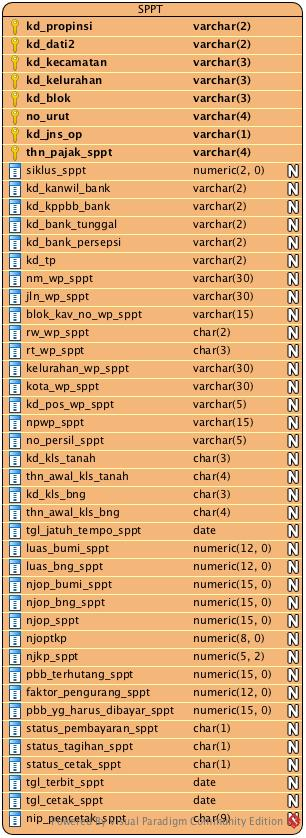
\includegraphics[width=0.5\textwidth]{./resources/struktur-tabel-sppt}
	\caption{Struktur Tabel SPPT}
	\label{fig:struktur-tabel-sppt}
\end{figure}

Penekanan pada tabel ini hanya ada pada beberapa \textit{field} atau kolom saja, yaitu pada \textit{field} atau kolom berikut :

\begin{itemize}
	\item Nomor Objek Pajak, yang terdiri dari \textit{field} atau kolom \texttt{kd\_propinsi}, \texttt{kd\_dati2}, \texttt{kd\_kecamatan}, \texttt{kd\_kelurahan}, \texttt{kd\_blok}, \texttt{no\_urut}, dan \texttt{kd\_jns\_op}.
	\item Tahun pajak pada \textit{field} atau kolom \texttt{thn\_pajak\_sppt}.
	\item Nama wajib pajak pada \textit{field} atau kolom \texttt{nm\_wp\_sppt}
	\item Besarnya pajak terhutang pada \textit{field} atau kolom \texttt{pbb\_yg\_harus\_dibayar\_sppt}
	\item Status pembayaran pada \textit{field} atau kolom \texttt{status\_pembayaran\_sppt}
\end{itemize}

\section{Tabel DAT\_OBJEK\_PAJAK}

Tabel \texttt{DAT\_OBJEK\_PAJAK}, digunakan untuk menampilkan informasi mengenai objek pajak seperti alamat, luas bumi dan bangunan, serta Nilai Jual Objek Bumi dan Bangunan. Struktur tabel dari \texttt{DAT\_OBJEK\_PAJAK} adalah seperti pada gambar \ref{fig:struktur-tabel-dat-op} berikut ini :

\begin{figure}[H]
	\centering
	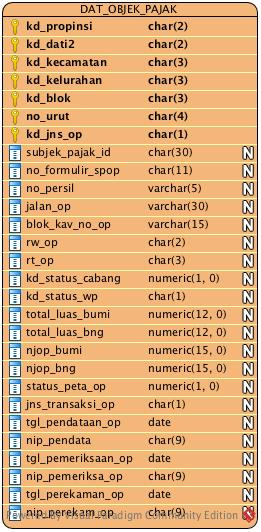
\includegraphics[width=0.5\textwidth]{./resources/struktur-tabel-dat-op}
	\caption{Struktur Tabel \texttt{DAT\_OBJEK\_PAJAK}}
	\label{fig:struktur-tabel-dat-op}
\end{figure}

\section{Tabel DAT\_SUBJEK\_PAJAK}

Tabel \texttt{DAT\_SUBJEK\_PAJAK} ini digunakan untuk menampilkan informasi mengenai subjek pajaknya seperti nama dan alamatnya. Struktur tabel dari \texttt{DAT\_SUBJEK\_PAJAK} ini adalah seperti pada gambar \ref{fig:struktur-tabel-dat-sp} berikut ini :

\begin{figure}[H]
	\centering
	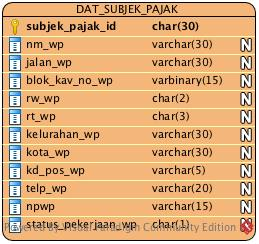
\includegraphics[width=0.5\textwidth]{./resources/struktur-tabel-dat-sp}
	\label{fig:struktur-tabel-dat-sp}
	\caption{Struktur Tabel \texttt{DAT\_SUBJEK\_PAJAK}}
\end{figure}

\section{Tabel REF\_KECAMATAN}

Untuk tabel \texttt{REF\_KECAMATAN} digunakan hanya untuk menampilkan informasi nama Kecamatan dimana objek berada. Struktur tabel untuk \texttt{REF\_KECAMATAN} ini seperti terlihat pada gambar \ref{fig:struktur-tabel-ref-kec} berikut ini :

\begin{figure}[H]
	\centering
	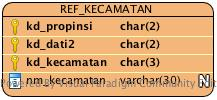
\includegraphics[width=0.5\textwidth]{./resources/struktur-tabel-ref-kec}
	\label{fig:struktur-tabel-ref-kec}
	\caption{Struktur Tabel \texttt{REF\_KECAMATAN}}
\end{figure}

\section{Tabel REF\_KELURAHAN}

Tabel \texttt{REF\_KELURAHAN} pun digunakan hanya untuk menampilkan nama Kelurahan/Desa dimana objek pajak berada. Struktur tabel \texttt{REF\_KELURAHAN} ini seperti terlihat pada gambar \ref{fig:struktur-tabel-ref-kel} berikut ini :

\begin{figure}[H]
	\centering
	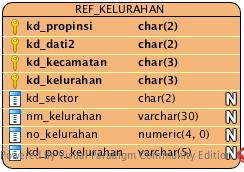
\includegraphics[width=0.5\textwidth]{./resources/struktur-tabel-ref-kel}
	\label{fig:struktur-tabel-ref-kel}
	\caption{Struktur Tabel \texttt{REF\_KELURAHAN}}
\end{figure}